
\section{Analyses statistiques et \\visualisation de données}



\begin{frame}{Analyse statistique}

  \begin{block}{Analyse statistique}
    \medskip
      \begin{itemize}
        \item<+-> Tirer de l'information des données dans l'objectif de \textbf{prendre des décisions}
        \item<+-> Identifier les tendances et les relations entre les différentes variables
        \item<+-> Statistiques : des méthodes mathématiques utilisées pour collecter, analyser et interpréter des données
        \item<+-> Les statistiques incluent la probabilité théorique, l'estimation des moyennes et des médianes, les tests de hypothèses, etc.
      \end{itemize}
  \end{block}
\end{frame}

\begin{frame}{Analyse statistique}
  \begin{block}{Objectifs}
    \medskip
    \begin{itemize}
      \item<+-> Tirer des insights des données pour prendre des décisions
      \item<+-> Identifier tendances et relations entre variables
    \end{itemize}
  \end{block}

  \onslide<3->{
    \begin{block}{Définition}
      \medskip
      \begin{itemize}
        \item<3-> Méthodes mathématiques pour collecter, analyser et interpréter des données
        \item<4-> Deux branches principales :
        \begin{enumerate}
          \item \textbf{Descriptive} : décrire les données (moyennes, graphiques)
          \item \textbf{Inférentielle} : généraliser à partir d'un échantillon
        \end{enumerate}
      \end{itemize}
    \end{block}
  }

  \onslide<5->{
    \begin{exampleblock}{Exemple concret}
      \medskip
      Un supermarché utilise la moyenne des ventes pour ajuster ses stocks
    \end{exampleblock}
  }
\end{frame}

\begin{frame}{Concepts statistiques essentiels}
  \begin{enumerate}
    \item<+-> \textbf{Mesures de tendance centrale :}
    \begin{itemize}
      \item Moyenne (sensible aux extrêmes)
      \item Médiane (robuste aux extrêmes)
    \end{itemize}

    \item<+-> \textbf{Mesures de dispersion :}
    \begin{itemize}
      \item Écart-type : variabilité autour de la moyenne
      \item Intervalle interquartile (IQR) : moins sensible aux extrêmes
    \end{itemize}

    \item<+-> \textbf{Corrélation vs causalité :}
    \begin{itemize}
      \item Exemple : ``Plus il y a de glaces vendues, plus il y a de noyades'' \\ $\Rightarrow$ corrélation $\neq$ causalité !
    \end{itemize}

    \item<+-> \textbf{Tests d'hypothèses :}
    \begin{itemize}
      \item Tester si un résultat est significatif (ex : un nouveau médicament est-il efficace ?)
    \end{itemize}
  \end{enumerate}
\end{frame}

\begin{frame}{Applications industrielles}
  \begin{block}{Domaines d'application}
    \medskip
    \begin{itemize}
      \item<+-> \textbf{Marketing} : segmentation client, A/B testing
      \item<+-> \textbf{Finance} : modélisation des risques, détection de fraudes
      \item<+-> \textbf{Santé} : études cliniques, analyse de données médicales
    \end{itemize}
  \end{block}

  \onslide<4->{
    \begin{alertblock}{Pièges à éviter}
      \medskip
      \begin{enumerate}
        \item Biais dans les données (échantillon non représentatif)
        \item Surinterprétation (corrélation $\neq$ causalité)
        \item Données de mauvaise qualité (manquantes, bruitées)
      \end{enumerate}
    \end{alertblock}
  }

  \onslide<5->{
    \begin{block}{Bonnes pratiques}
      \medskip
      \begin{itemize}
        \item Vérifier la qualité des données avant analyse
        \item Choisir les bonnes métriques (moyenne vs médiane)
        \item Documenter et itérer sur les modèles
      \end{itemize}
    \end{block}
  }
\end{frame}

\begin{frame}{Outils pour l'analyse statistique}
  \begin{block}{Outils disponibles}
    \medskip
    \begin{itemize}
      \item<+-> \textbf{Excel/Google Sheets} : fonctions de base, graphiques
      \item<+-> \textbf{Python/R} : Pandas, Scikit-learn, Statsmodels
      \item<+-> \textbf{Tableau/Power BI} : visualisation interactive
    \end{itemize}
  \end{block}

  \onslide<4->{
    \begin{exampleblock}{Exemple concret : Analyse des ventes}
      \medskip
      \begin{enumerate}
        \item Données : ventes mensuelles + prix/promotions/saison
        \item Analyse descriptive : moyennes, graphiques temporels
        \item Modélisation : régression linéaire pour prédire les ventes
        \item Résultats actionnables : ``Les promotions augmentent les ventes de 15\%''
      \end{enumerate}
    \end{exampleblock}
  }
\end{frame}

\begin{frame}{Visualisation de données}

\end{frame}


\begin{frame}{Visualisation de données}
  \begin{block}{Visualisation}
    \medskip
    ``La visualisation est un processus \textcolor{blue}{cognitif} qui permet de former une \textcolor{blue}{image mentale} pour découvrir, expliquer et \textcolor{red}{prendre des décisions}.''
  \end{block}

  \onslide<2>{
    \begin{block}{Visualisation de données}
      \medskip
      ``La visualisation de données est la représentation visuelle informatisée de données \textcolor{blue}{pour amplifier} la cognition.''
    \end{block}
    
    \bigskip
    Source : \href{https://maelfabien.github.io/machinelearning/Dataviz/}{\underline{maelfabien.github.io}}
  }
\end{frame}

\begin{frame}{Intérêt de la visualisation de données}
  \centering
  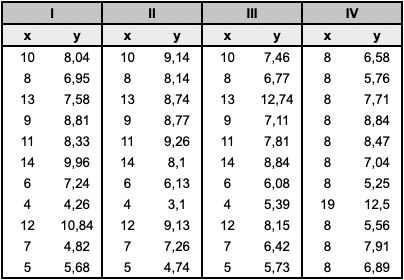
\includegraphics[scale=.5]{img/intro/anscombe.png}

  Anscombe's quartet
\end{frame}

\begin{frame}{Intérêt de la visualisation de données}
  \begin{center}
    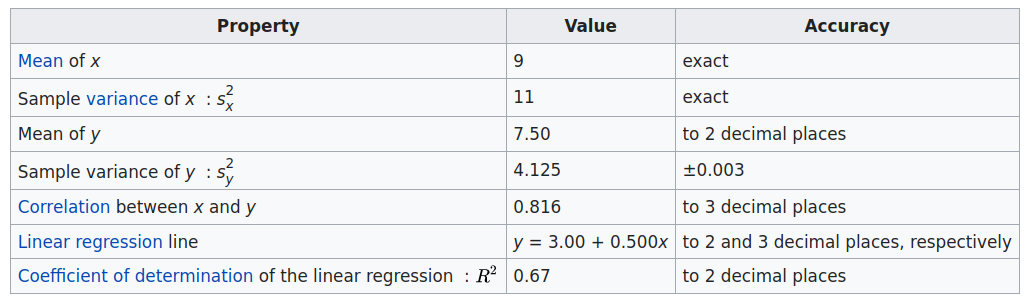
\includegraphics[width=\textwidth]{img/intro/anscombe_wikipedia.png}
    
    Anscombe's quartet
  \end{center}

  \bigskip
  \bigskip
  \bigskip
  \bigskip
  \footnotesize
  Source : Wikipedia
\end{frame}

\begin{frame}{Intérêt de la visualisation de données}
  \begin{center}
    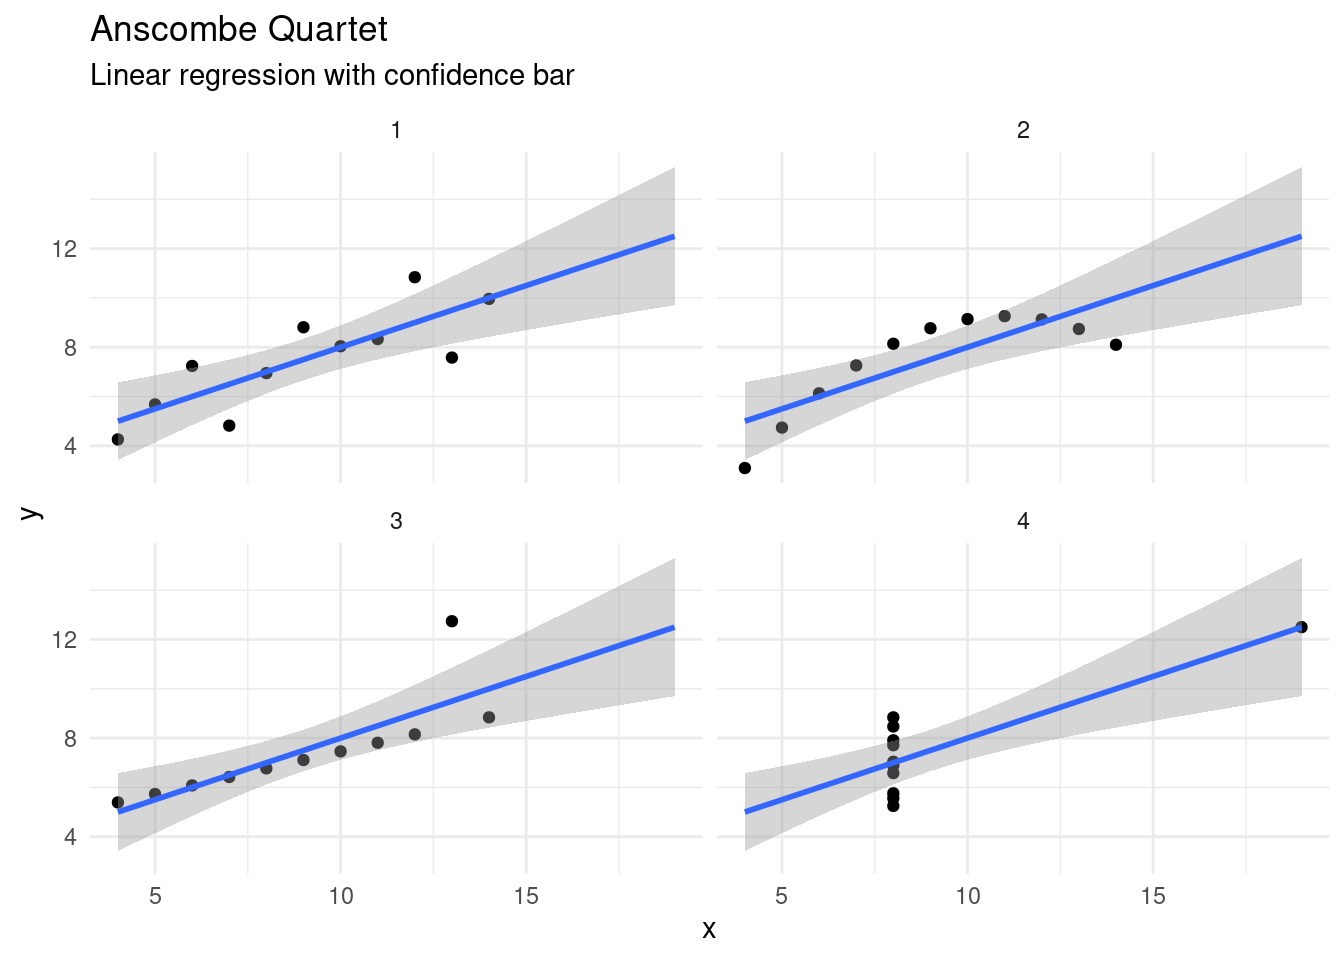
\includegraphics[width=.7\textwidth]{img/intro/Anscombe_Lm_Points-1.png}
  \end{center}

  \footnotesize
  Source : Wikipedia
\end{frame}

